% Options for packages loaded elsewhere
\PassOptionsToPackage{unicode}{hyperref}
\PassOptionsToPackage{hyphens}{url}
%
\documentclass[
]{article}
\usepackage{lmodern}
\usepackage{amssymb,amsmath}
\usepackage{ifxetex,ifluatex}
\ifnum 0\ifxetex 1\fi\ifluatex 1\fi=0 % if pdftex
  \usepackage[T1]{fontenc}
  \usepackage[utf8]{inputenc}
  \usepackage{textcomp} % provide euro and other symbols
\else % if luatex or xetex
  \usepackage{unicode-math}
  \defaultfontfeatures{Scale=MatchLowercase}
  \defaultfontfeatures[\rmfamily]{Ligatures=TeX,Scale=1}
\fi
% Use upquote if available, for straight quotes in verbatim environments
\IfFileExists{upquote.sty}{\usepackage{upquote}}{}
\IfFileExists{microtype.sty}{% use microtype if available
  \usepackage[]{microtype}
  \UseMicrotypeSet[protrusion]{basicmath} % disable protrusion for tt fonts
}{}
\makeatletter
\@ifundefined{KOMAClassName}{% if non-KOMA class
  \IfFileExists{parskip.sty}{%
    \usepackage{parskip}
  }{% else
    \setlength{\parindent}{0pt}
    \setlength{\parskip}{6pt plus 2pt minus 1pt}}
}{% if KOMA class
  \KOMAoptions{parskip=half}}
\makeatother
\usepackage{xcolor}
\IfFileExists{xurl.sty}{\usepackage{xurl}}{} % add URL line breaks if available
\IfFileExists{bookmark.sty}{\usepackage{bookmark}}{\usepackage{hyperref}}
\hypersetup{
  pdftitle={DATA 101 Project\_1},
  pdfauthor={Ana Ortez-Rivera, Tiffany King, Jennifer Johnson},
  hidelinks,
  pdfcreator={LaTeX via pandoc}}
\urlstyle{same} % disable monospaced font for URLs
\usepackage[margin=1in]{geometry}
\usepackage{color}
\usepackage{fancyvrb}
\newcommand{\VerbBar}{|}
\newcommand{\VERB}{\Verb[commandchars=\\\{\}]}
\DefineVerbatimEnvironment{Highlighting}{Verbatim}{commandchars=\\\{\}}
% Add ',fontsize=\small' for more characters per line
\usepackage{framed}
\definecolor{shadecolor}{RGB}{248,248,248}
\newenvironment{Shaded}{\begin{snugshade}}{\end{snugshade}}
\newcommand{\AlertTok}[1]{\textcolor[rgb]{0.94,0.16,0.16}{#1}}
\newcommand{\AnnotationTok}[1]{\textcolor[rgb]{0.56,0.35,0.01}{\textbf{\textit{#1}}}}
\newcommand{\AttributeTok}[1]{\textcolor[rgb]{0.77,0.63,0.00}{#1}}
\newcommand{\BaseNTok}[1]{\textcolor[rgb]{0.00,0.00,0.81}{#1}}
\newcommand{\BuiltInTok}[1]{#1}
\newcommand{\CharTok}[1]{\textcolor[rgb]{0.31,0.60,0.02}{#1}}
\newcommand{\CommentTok}[1]{\textcolor[rgb]{0.56,0.35,0.01}{\textit{#1}}}
\newcommand{\CommentVarTok}[1]{\textcolor[rgb]{0.56,0.35,0.01}{\textbf{\textit{#1}}}}
\newcommand{\ConstantTok}[1]{\textcolor[rgb]{0.00,0.00,0.00}{#1}}
\newcommand{\ControlFlowTok}[1]{\textcolor[rgb]{0.13,0.29,0.53}{\textbf{#1}}}
\newcommand{\DataTypeTok}[1]{\textcolor[rgb]{0.13,0.29,0.53}{#1}}
\newcommand{\DecValTok}[1]{\textcolor[rgb]{0.00,0.00,0.81}{#1}}
\newcommand{\DocumentationTok}[1]{\textcolor[rgb]{0.56,0.35,0.01}{\textbf{\textit{#1}}}}
\newcommand{\ErrorTok}[1]{\textcolor[rgb]{0.64,0.00,0.00}{\textbf{#1}}}
\newcommand{\ExtensionTok}[1]{#1}
\newcommand{\FloatTok}[1]{\textcolor[rgb]{0.00,0.00,0.81}{#1}}
\newcommand{\FunctionTok}[1]{\textcolor[rgb]{0.00,0.00,0.00}{#1}}
\newcommand{\ImportTok}[1]{#1}
\newcommand{\InformationTok}[1]{\textcolor[rgb]{0.56,0.35,0.01}{\textbf{\textit{#1}}}}
\newcommand{\KeywordTok}[1]{\textcolor[rgb]{0.13,0.29,0.53}{\textbf{#1}}}
\newcommand{\NormalTok}[1]{#1}
\newcommand{\OperatorTok}[1]{\textcolor[rgb]{0.81,0.36,0.00}{\textbf{#1}}}
\newcommand{\OtherTok}[1]{\textcolor[rgb]{0.56,0.35,0.01}{#1}}
\newcommand{\PreprocessorTok}[1]{\textcolor[rgb]{0.56,0.35,0.01}{\textit{#1}}}
\newcommand{\RegionMarkerTok}[1]{#1}
\newcommand{\SpecialCharTok}[1]{\textcolor[rgb]{0.00,0.00,0.00}{#1}}
\newcommand{\SpecialStringTok}[1]{\textcolor[rgb]{0.31,0.60,0.02}{#1}}
\newcommand{\StringTok}[1]{\textcolor[rgb]{0.31,0.60,0.02}{#1}}
\newcommand{\VariableTok}[1]{\textcolor[rgb]{0.00,0.00,0.00}{#1}}
\newcommand{\VerbatimStringTok}[1]{\textcolor[rgb]{0.31,0.60,0.02}{#1}}
\newcommand{\WarningTok}[1]{\textcolor[rgb]{0.56,0.35,0.01}{\textbf{\textit{#1}}}}
\usepackage{graphicx,grffile}
\makeatletter
\def\maxwidth{\ifdim\Gin@nat@width>\linewidth\linewidth\else\Gin@nat@width\fi}
\def\maxheight{\ifdim\Gin@nat@height>\textheight\textheight\else\Gin@nat@height\fi}
\makeatother
% Scale images if necessary, so that they will not overflow the page
% margins by default, and it is still possible to overwrite the defaults
% using explicit options in \includegraphics[width, height, ...]{}
\setkeys{Gin}{width=\maxwidth,height=\maxheight,keepaspectratio}
% Set default figure placement to htbp
\makeatletter
\def\fps@figure{htbp}
\makeatother
\setlength{\emergencystretch}{3em} % prevent overfull lines
\providecommand{\tightlist}{%
  \setlength{\itemsep}{0pt}\setlength{\parskip}{0pt}}
\setcounter{secnumdepth}{-\maxdimen} % remove section numbering

\title{DATA 101 Project\_1}
\author{Ana Ortez-Rivera, Tiffany King, Jennifer Johnson}
\date{8/10/2020}

\begin{document}
\maketitle

\begin{Shaded}
\begin{Highlighting}[]
\KeywordTok{library}\NormalTok{(git2r)}
\KeywordTok{library}\NormalTok{(usethis)}
\end{Highlighting}
\end{Shaded}

\hypertarget{racial-demographics-at-for-profit-and-not-for-profit-educational-institutions}{%
\section{\texorpdfstring{\textbf{Racial Demographics at For-Profit and
Not-For-Profit Educational
Institutions}}{Racial Demographics at For-Profit and Not-For-Profit Educational Institutions}}\label{racial-demographics-at-for-profit-and-not-for-profit-educational-institutions}}

\hypertarget{until-we-get-equality-in-education-we-wont-have-an-equal-society.}{%
\subsubsection{\texorpdfstring{\emph{``Until we get equality in
education, we won't have an equal
society.''}}{``Until we get equality in education, we won't have an equal society.''}}\label{until-we-get-equality-in-education-we-wont-have-an-equal-society.}}

\hypertarget{supreme-court-justice-sonia-sotomayor}{%
\paragraph{\textasciitilde{} Supreme Court Justice Sonia
Sotomayor}\label{supreme-court-justice-sonia-sotomayor}}

\hypertarget{topic-background}{%
\subsection{\texorpdfstring{\textbf{Topic
Background}}{Topic Background}}\label{topic-background}}

Each of our team members originally selected a few datasets that we
compared as a group. Our group decided to explore a dataset Ana found
related to the topic of racial and ethnic diversity at two-year and
four-year colleges and universities in the United States. We initally
thought to compare diversity at two-year community colleges versus
4-year schools and also were curious about the variations in diversity
between the two that could be found comparatively across the country.

As we were exploring the dataset we identified a number of named
colleges and universities that are known as ``for-profit'' institutions.
Some of these institutions have been the subject of recent lawsuits
regarding predatory (Halperin, 2020; Legal Services Center, 2020;
Redman, 2020). The high number of current lawsuits regarding for-profit
colleges' predatory behaviors are a result of the actions of current
Education Secretary Betsy DeVos. In 2019, DeVos ``repealed an Obama-era
regulation that sought to crack down on for-profit colleges and
universities that produced graduates with no meaningful job prospects
and mountains of student debt they could not hope to repay'' (Green,
2019. para. 1). Another action that DeVos took was to deny debt
forgiveness to students who had been prey to for-profit predatory
educational institutions (Lobosco, 2019; Turner, 2019). We were aware of
past and recent news articles describing the marketing strategies of
these colleges that were aimed at students of color, low-income
students, immigrant communities and students who are first in their
family to go to college (Bonadies et al.~2018; Conti, 2019; Voorhees,
2019). Previous studies have found that loan debt is higher for students
who have attended For-Profit institutions, which disproportionately
affects students of color.

\begin{figure}
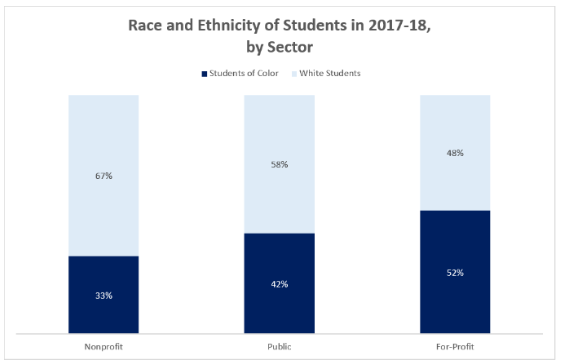
\includegraphics[width=0.75\linewidth]{chart_2} \caption{**Race and For-Profits**}\label{fig:pressure2}
\end{figure}

(Body, 2019)

\begin{figure}
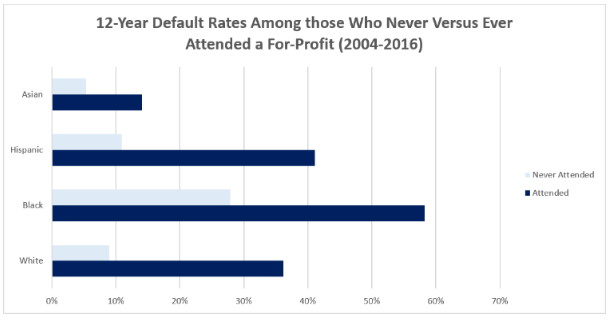
\includegraphics[width=0.75\linewidth]{chart_1} \caption{**Loan Default Rates at For-Profits**}\label{fig:pressure3}
\end{figure}

(Body, 2019)

Despite their high cost, For-profit institutions have a lower graduation
rate and employment rate than non-profit institutions.

\begin{figure}
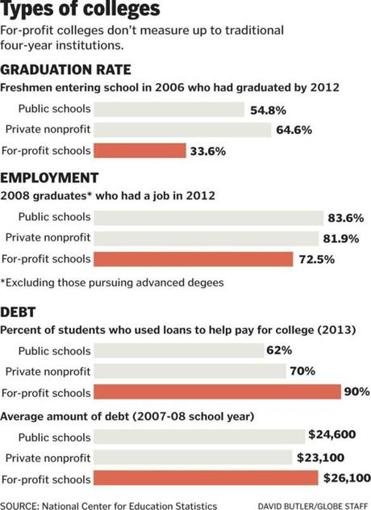
\includegraphics[width=0.5\linewidth]{chart_3} \caption{**For-Profit Graduation & Employment Rates**}\label{fig:pressure4}
\end{figure}

(Lopez, 2015)

We will examine our dataset and explore possible consistencies and/or
inconsistencies with these previous reports.

\hypertarget{initial-questions}{%
\subsection{\texorpdfstring{\textbf{Initial
Questions}}{Initial Questions}}\label{initial-questions}}

\begin{enumerate}
\def\labelenumi{\arabic{enumi}.}
\item
  How do racial and ethnic demographics vary between not-for-profit
  institutions and for-profit colleges in our dataset?
\item
  In our dataset, do the For-Profit Institutions have a higher
  proportion of students of color than other community colleges and
  four-year colleges, thus providing support to the argument that
  For-Profit colleges target students of color for enrollment?
\end{enumerate}

\hypertarget{definitions}{%
\subsection{\texorpdfstring{\textbf{Definitions}:}{Definitions:}}\label{definitions}}

\textbf{For-Profit Institutions}: For-profit institutions are defined by
the way that ``revenue earned by the school is invested''. For-profit
colleges have investors who want to make a profit. Their operations
management is determined in part on maximizing the return profit for
investors. ``Money earned by the shcool may be used to pay out investors
and award boneuses to executives, as well as sustain the operation's
profitability through aggressive marketing and recruitment strategies''
(TBS Staff, 2019, para. 8)

\textbf{Not-for Profit Institutions}: Non-profit colleges can be either
public or private. Regardless of whether the school is public or
private, non-profit colleges must ``reinvest the money earned through
enrollment into the educational mission'' (TBS Staff, 2019, para. 8).

\hypertarget{webscraping-and-randomly-selecting-sample-of-35-for-profit-colleges}{%
\subsection{\texorpdfstring{\textbf{Webscraping and Randomly Selecting
Sample of 35 For-Profit
Colleges}}{Webscraping and Randomly Selecting Sample of 35 For-Profit Colleges}}\label{webscraping-and-randomly-selecting-sample-of-35-for-profit-colleges}}

Our dataset did not include information on whether colleges were
for-profit.

In order to determine which of the schools on our list were for-profit
institutions, we decided to find a website with a list of for-profit
institutions, scrape the data from that website, to create a second
dataset with a list of for profit schools.

\hypertarget{following-web-scraping-tutorial-to-scrape-wikipedia-website}{%
\subsubsection{Following Web-Scraping Tutorial to Scrape Wikipedia
Website}\label{following-web-scraping-tutorial-to-scrape-wikipedia-website}}

\hypertarget{loading-libraries}{%
\subsubsection{Loading Libraries}\label{loading-libraries}}

\begin{Shaded}
\begin{Highlighting}[]
\CommentTok{#Loading the rvest package}
\KeywordTok{library}\NormalTok{(}\StringTok{'rvest'}\NormalTok{)}
\end{Highlighting}
\end{Shaded}

\begin{verbatim}
## Loading required package: xml2
\end{verbatim}

\begin{Shaded}
\begin{Highlighting}[]
\KeywordTok{library}\NormalTok{(tidyverse)}
\end{Highlighting}
\end{Shaded}

\begin{verbatim}
## -- Attaching packages ---------------------------------------------------------------------------- tidyverse 1.3.0 --
\end{verbatim}

\begin{verbatim}
## v ggplot2 3.3.1     v purrr   0.3.4
## v tibble  3.0.1     v dplyr   1.0.0
## v tidyr   1.1.0     v stringr 1.4.0
## v readr   1.3.1     v forcats 0.5.0
\end{verbatim}

\begin{verbatim}
## Warning: package 'dplyr' was built under R version 4.0.2
\end{verbatim}

\begin{verbatim}
## -- Conflicts ------------------------------------------------------------------------------- tidyverse_conflicts() --
## x dplyr::filter()         masks stats::filter()
## x readr::guess_encoding() masks rvest::guess_encoding()
## x purrr::is_empty()       masks git2r::is_empty()
## x dplyr::lag()            masks stats::lag()
## x purrr::pluck()          masks rvest::pluck()
## x dplyr::pull()           masks git2r::pull()
## x purrr::when()           masks git2r::when()
\end{verbatim}

\begin{Shaded}
\begin{Highlighting}[]
\KeywordTok{library}\NormalTok{(dplyr)}
\end{Highlighting}
\end{Shaded}

\begin{Shaded}
\begin{Highlighting}[]
\CommentTok{#Specifying the url for desired website to be scraped}
\NormalTok{url <-}\StringTok{ 'https://en.wikipedia.org/wiki/List_of_for-profit_universities_and_colleges'}

\CommentTok{#Reading the HTML code from the website}
\NormalTok{webpage <-}\StringTok{ }\KeywordTok{read_html}\NormalTok{(url)}

\CommentTok{#Using CSS selectors to scrape the rankings section}
\NormalTok{for_profit_html <-}\StringTok{ }\KeywordTok{html_nodes}\NormalTok{(webpage,}\StringTok{'li a'}\NormalTok{)}
\CommentTok{#Converting the ranking data to text}
\NormalTok{for_profit <-}\StringTok{ }\KeywordTok{html_text}\NormalTok{(for_profit_html)}

\CommentTok{#Let's have a look at the rankings}
\KeywordTok{head}\NormalTok{(for_profit)}
\end{Highlighting}
\end{Shaded}

\begin{verbatim}
## [1] "1 In the United States"                                          
## [2] "2 Distance education (online)"                                   
## [3] "3 Outside the United States"                                     
## [4] "3.1 Closed or merged"                                            
## [5] "4 For-profit colleges that became non-profit colleges"           
## [6] "4.1 For-profit colleges that became non-profit colleges (closed)"
\end{verbatim}

\hypertarget{viewing-new-index}{%
\subsubsection{Viewing new index}\label{viewing-new-index}}

\begin{Shaded}
\begin{Highlighting}[]
\CommentTok{# for_profit}
\end{Highlighting}
\end{Shaded}

\begin{Shaded}
\begin{Highlighting}[]
\NormalTok{for_profit_new <-}\StringTok{ }\NormalTok{for_profit[}\DecValTok{25}\OperatorTok{:}\DecValTok{215}\NormalTok{]}
\KeywordTok{head}\NormalTok{(for_profit_new)}
\end{Highlighting}
\end{Shaded}

\begin{verbatim}
## [1] "Academy of Art University"           
## [2] "American Career College"             
## [3] "American College of Education"       
## [4] "American InterContinental University"
## [5] "Career Education Corporation"        
## [6] "American Military University"
\end{verbatim}

\hypertarget{cleaning-our-for-profit-list}{%
\subsubsection{Cleaning our for-profit
list}\label{cleaning-our-for-profit-list}}

\begin{Shaded}
\begin{Highlighting}[]
\NormalTok{for_profit_new[}\DecValTok{167}\OperatorTok{:}\DecValTok{168}\NormalTok{] <-}\StringTok{ }\OtherTok{NA}
\NormalTok{for_profit_new}
\end{Highlighting}
\end{Shaded}

\begin{verbatim}
##   [1] "Academy of Art University"                             
##   [2] "American Career College"                               
##   [3] "American College of Education"                         
##   [4] "American InterContinental University"                  
##   [5] "Career Education Corporation"                          
##   [6] "American Military University"                          
##   [7] "American National University"                          
##   [8] "American University"                                   
##   [9] "National American University"                          
##  [10] "American Public University"                            
##  [11] "American Sentinel University"                          
##  [12] "Ancora Education"                                      
##  [13] "Antonelli College"                                     
##  [14] "Art Institutes"                                        
##  [15] "ASA College"                                           
##  [16] "Aspen University"                                      
##  [17] "Bay State College"                                     
##  [18] "Berkeley College"                                      
##  [19] "University of California, Berkeley"                    
##  [20] "Berklee College of Music"                              
##  [21] "Berkeley College at Yale University"                   
##  [22] "Blair College"                                         
##  [23] "Colorado Springs, Colorado"                            
##  [24] "Blue Cliff College"                                    
##  [25] "Bradford School (Columbus)"                            
##  [26] "Columbus, Ohio"                                        
##  [27] "Bradford School (Pittsburgh)"                          
##  [28] "Pittsburgh, Pennsylvania"                              
##  [29] "Branford Hall Career Institute"                        
##  [30] "Broadview University"                                  
##  [31] "Brookline College"                                     
##  [32] "Bryant & Stratton College"                             
##  [33] "Burrell College of Osteopathic Medicine"               
##  [34] "California Miramar University"                         
##  [35] "California Northstate University College of Medicine"  
##  [36] "Capella University"                                    
##  [37] "Centura College"                                       
##  [38] "Chamberlain College of Nursing"                        
##  [39] "Adtalem"                                               
##  [40] "Charleston School of Law"                              
##  [41] "Charter College"                                       
##  [42] "The College of Westchester"                            
##  [43] "West Chester University"                               
##  [44] "West Chester, Pennsylvania"                            
##  [45] "Colorado Technical University"                         
##  [46] "Career Education Corporation"                          
##  [47] "Columbia Southern University"                          
##  [48] "Columbia University"                                   
##  [49] "Conservatory of Recording Arts and Sciences"           
##  [50] "Cortiva Institute"                                     
##  [51] "Daymar College"                                        
##  [52] "DeVry University"                                      
##  [53] "Keller School of Management"                           
##  [54] "DigiPen Institute of Technology"                       
##  [55] "Redmond, Washington"                                   
##  [56] "Eagle Gate College"                                    
##  [57] "ECPI University"                                       
##  [58] "Engine City Technical Institute"                       
##  [59] "South Plainfield, New Jersey"                          
##  [60] "Fashion Institute of Design & Merchandising"           
##  [61] "Fashion Institute of Technology"                       
##  [62] "New York City"                                         
##  [63] "Five Towns College"                                    
##  [64] "Dix Hills, New York"                                   
##  [65] "Florida Career College"                                
##  [66] "Florida Coastal School of Law"                         
##  [67] "InfiLaw System"                                        
##  [68] "Florida Metropolitan University"                       
##  [69] "Florida National University"                           
##  [70] "Hialeah, Florida"                                      
##  [71] "Fortis College"                                        
##  [72] "Fox College"                                           
##  [73] "Chicago metropolitan area"                             
##  [74] "Bedford Park"                                          
##  [75] "Tinley Park"                                           
##  [76] "Full Sail University"                                  
##  [77] "Winter Park, Florida"                                  
##  [78] "Georgia Medical Institute"                             
##  [79] "Medical College of Georgia"                            
##  [80] "Augusta University"                                    
##  [81] "Grand Canyon University"                               
##  [82] "Grantham University"                                   
##  [83] "Kansas City, Missouri"                                 
##  [84] "Hamilton College"                                      
##  [85] "Hamilton College"                                      
##  [86] "Hamilton University"                                   
##  [87] "Harris School of Business"                             
##  [88] "Idaho College of Osteopathic Medicine"                 
##  [89] "International Education Corporation"                   
##  [90] "Las Vegas College"                                     
##  [91] "Laureate International Universities"                   
##  [92] "Walden University"                                     
##  [93] "Lincoln Tech"                                          
##  [94] "Lincoln University"                                    
##  [95] "Los Angeles Film School"                               
##  [96] "McCann School of Business and Technology"              
##  [97] "Miami International University of Art and Design"      
##  [98] "Mildred Elley"                                         
##  [99] "Miller-Motte"                                          
## [100] "Minneapolis Business College"                          
## [101] "Roseville, Minnesota"                                  
## [102] "Monroe College"                                        
## [103] "Mountain West College"                                 
## [104] "National American University"                          
## [105] "Mall of America"                                       
## [106] "American University"                                   
## [107] "National College"                                      
## [108] "National Institute of Technology (United States)"      
## [109] "National Institutes of Technology"                     
## [110] "National Paralegal College"                            
## [111] "National University College"                           
## [112] "Neumont University"                                    
## [113] "NewSchool of Architecture and Design"                  
## [114] "The New School"                                        
## [115] "Northwestern College"                                  
## [116] "Northwestern University"                               
## [117] "Ohio Business College"                                 
## [118] "Olympia Career Training Institute"                     
## [119] "Pacific College of Oriental Medicine"                  
## [120] "Parks College"                                         
## [121] "Paier College of Art"                                  
## [122] "Pennco Tech"                                           
## [123] "Pima Medical Institute"                                
## [124] "Pinnacle Career Institute"                             
## [125] "Pioneer Pacific College"                               
## [126] "Pittsburgh Technical Institute"                        
## [127] "Oakdale, Pennsylvania"                                 
## [128] "Cranberry Township, Butler County, Pennsylvania"       
## [129] "Platt College"                                         
## [130] "Plaza College"                                         
## [131] "Porter and Chester Institute"                          
## [132] "Post University"                                       
## [133] "LIU Post"                                              
## [134] "Potomac College"                                       
## [135] "Provo College"                                         
## [136] "Rasmussen College"                                     
## [137] "Recording Radio Film Connection"                       
## [138] "Redstone College"                                      
## [139] "Rocky Mountain College of Art and Design"              
## [140] "Lakewood, Colorado"                                    
## [141] "Rocky Mountain University of Health Professions"       
## [142] "Rocky Vista University College of Osteopathic Medicine"
## [143] "SAE Institute"                                         
## [144] "Salem International University"                        
## [145] "Salem, West Virginia"                                  
## [146] "Salter College"                                        
## [147] "San Joaquin Valley College"                            
## [148] "Schiller International University"                     
## [149] "School of Visual Arts"                                 
## [150] "Seacoast Career Schools"                               
## [151] "South College"                                         
## [152] "South University"                                      
## [153] "Southern University"                                   
## [154] "University of the South"                               
## [155] "Southern Careers Institute"                            
## [156] "Southern States University"                            
## [157] "Southwestern College"                                  
## [158] "Southwestern University"                               
## [159] "Lincoln University"                                    
## [160] "Spartan College of Aeronautics and Technology"         
## [161] "Specs Howard School of Media Arts"                     
## [162] "Spencerian College"                                    
## [163] "Stevens-Henager College"                               
## [164] "Stratford University"                                  
## [165] "Strayer University"                                    
## [166] "Sullivan University"                                   
## [167] NA                                                      
## [168] NA                                                      
## [169] "UEI College"                                           
## [170] "United States University"                              
## [171] "Universal Technical Institute"                         
## [172] "University of Advancing Technology"                    
## [173] "University of Phoenix"                                 
## [174] "University of the Potomac"                             
## [175] "U.S. Career Institute"                                 
## [176] "Fort Collins, Colorado"                                
## [177] "Vista College"                                         
## [178] "Walden University"                                     
## [179] "Waldorf College"                                       
## [180] "Washington Technology University"                      
## [181] "West Coast University"                                 
## [182] "Western Business College"                              
## [183] "Western International University"                      
## [184] "Apollo Group"                                          
## [185] "Western State College of Law"                          
## [186] "Western State University College of Law"               
## [187] "Fullerton, California"                                 
## [188] "Western Governors University"                          
## [189] "Wood Tobé-Coburn School"                               
## [190] "New York City"                                         
## [191] "Wyoming Technical Institute (WyoTech)"
\end{verbatim}

\begin{Shaded}
\begin{Highlighting}[]
\NormalTok{final_for_profit <-}\StringTok{ }\KeywordTok{na.omit}\NormalTok{(for_profit_new)}
\end{Highlighting}
\end{Shaded}

\begin{Shaded}
\begin{Highlighting}[]
\CommentTok{#final_for_profit}
\NormalTok{ df <-}\KeywordTok{data_frame}\NormalTok{(final_for_profit)}
\end{Highlighting}
\end{Shaded}

\begin{verbatim}
## Warning: `data_frame()` is deprecated as of tibble 1.1.0.
## Please use `tibble()` instead.
## This warning is displayed once every 8 hours.
## Call `lifecycle::last_warnings()` to see where this warning was generated.
\end{verbatim}

\begin{Shaded}
\begin{Highlighting}[]
\NormalTok{df}
\end{Highlighting}
\end{Shaded}

\begin{verbatim}
## # A tibble: 189 x 1
##    final_for_profit                    
##    <chr>                               
##  1 Academy of Art University           
##  2 American Career College             
##  3 American College of Education       
##  4 American InterContinental University
##  5 Career Education Corporation        
##  6 American Military University        
##  7 American National University        
##  8 American University                 
##  9 National American University        
## 10 American Public University          
## # ... with 179 more rows
\end{verbatim}

The webscraping exercise produced a list of over 1,000 schools. We
decided to take a random sample of n=35 schools on that list, which also
appeared in our dataset. We selected 35 schools so that we would comply
with the Central Limit Theorem. The result of the randomization we ran
on the webscraped data is below. Each of us compared a portion of the
list with our dataset to ensure that all of our selections were present
on both lists. We ran multiple randomizations until we had a consistent
list with 35 schools appearing on both datasets. Some of the randomly
chosen schools had multiple locations, as is shown in the example set of
schools below. The final list of schools was geographically diverse.

\begin{Shaded}
\begin{Highlighting}[]
\KeywordTok{sample_n}\NormalTok{(df,}\DecValTok{35}\NormalTok{)}
\end{Highlighting}
\end{Shaded}

\begin{verbatim}
## # A tibble: 35 x 1
##    final_for_profit                    
##    <chr>                               
##  1 South College                       
##  2 Mountain West College               
##  3 Capella University                  
##  4 Seacoast Career Schools             
##  5 American InterContinental University
##  6 Bradford School (Pittsburgh)        
##  7 Redmond, Washington                 
##  8 U.S. Career Institute               
##  9 Waldorf College                     
## 10 New York City                       
## # ... with 25 more rows
\end{verbatim}

\hypertarget{jennifer}{%
\subsubsection{Jennifer}\label{jennifer}}

\begin{itemize}
\tightlist
\item
  Spencerian College

  \begin{itemize}
  \tightlist
  \item
    Spencerian College at Louisville (Ky.)
  \item
    Spencerian College at Lexington (Ky.
  \end{itemize}
\item
  Aspen University\\
\item
  American Public University

  \begin{itemize}
  \tightlist
  \item
    American Public University system
  \end{itemize}
\item
  Western International University\\
\item
  NewSchool of Architecture and Design\\
\item
  Schiller International University
\item
  National Paralegal College\\
\item
  West Coast University

  \begin{itemize}
  \tightlist
  \item
    West Coast University at Ontario
  \item
    West Coast University trasound Institute
  \item
    West Coast University at Dallas
  \item
    West Coast University at Miami
  \item
    West Coast University -Los Angeles
  \item
    West Coast University -Orange County
  \end{itemize}
\item
  Mildred Elley

  \begin{itemize}
  \tightlist
  \item
    Mildred Elley
  \item
    Mildred Elley at New York City
  \end{itemize}
\item
  Brookline College

  \begin{itemize}
  \tightlist
  \item
    Brookline College at Tucson
  \item
    Brookline College at Tempe (Ariz.)
  \item
    Brookline College at Albuquerque
  \item
    Brookline College at Phoenix
  \end{itemize}
\item
  Grand Canyon University
\end{itemize}

\hypertarget{ana}{%
\subsubsection{Ana}\label{ana}}

\begin{itemize}
\tightlist
\item
  Walden University
\item
  Blue Cliff College

  \begin{itemize}
  \tightlist
  \item
    Blue Cliff College at Metairie
  \item
    Blue Cliff College at Alexandria
  \item
    Blue Cliff College at Shreveport
  \item
    Blue Cliff College at Gulfport
  \end{itemize}
\item
  Neumont University\\
\item
  University of Pheonix
\item
  Stevens-Henager College\\
\item
  DeVry University\\
\item
  Pioneer Pacific College\\
\item
  Capella University\\
\item
  Grantham University\\
\item
  Stratford University\\
\item
  Redstone College\\
\item
  National College
\end{itemize}

\hypertarget{tiffany}{%
\subsubsection{Tiffany}\label{tiffany}}

\begin{itemize}
\tightlist
\item
  Strayer University\\
\item
  Lincoln Tech\\
\item
  Full Sail University\\
\item
  Rocky Mountain College of Art and Design\\
\item
  Minneapolis Business College\\
\item
  Fashion Institute of Design \& Merchandising\\
\item
  Paier College of Art
\item
  Vista College
\item
  Centura College\\
\item
  Rasmussen College
\item
  Redstone College\\
\item
  Fortis College\\
\item
  Bay State College
\end{itemize}

\hypertarget{data-wrangling-analysis}{%
\subsection{\texorpdfstring{\textbf{Data Wrangling \&
Analysis}}{Data Wrangling \& Analysis}}\label{data-wrangling-analysis}}

The dataset we chose to work with produced diversity counts at
institutions of higher learning in the United States. The datset was
retrieved from Kaggle, available here:
\url{https://www.kaggle.com/jessemostipak/college-tuition-diversity-and-pay?select=diversity_school.csv}

The entire dataset is composed of five separate .csv files addressing
school diversity, historical tuition rates, salary protential, the cost
of tuition in 2016 and the income of students compared to tuition. We
utilized the school diversity file only.

\hypertarget{setting-working-directory}{%
\subsubsection{Setting working
directory}\label{setting-working-directory}}

\begin{Shaded}
\begin{Highlighting}[]
\KeywordTok{setwd}\NormalTok{(}\StringTok{"/Users/anaortez-rivera/Desktop/Project_1_DATA101"}\NormalTok{) }
\NormalTok{diversity <-}\StringTok{ }\KeywordTok{read_csv}\NormalTok{(}\StringTok{"diversity_school_2.csv"}\NormalTok{)}
\end{Highlighting}
\end{Shaded}

\begin{verbatim}
## Parsed with column specification:
## cols(
##   name = col_character(),
##   total_enrollment = col_double(),
##   state = col_character(),
##   category = col_character(),
##   enrollment = col_double()
## )
\end{verbatim}

\hypertarget{viewing-data}{%
\subsubsection{Viewing data}\label{viewing-data}}

\begin{Shaded}
\begin{Highlighting}[]
\KeywordTok{head}\NormalTok{(diversity)}
\end{Highlighting}
\end{Shaded}

\begin{verbatim}
## # A tibble: 6 x 5
##   name                total_enrollment state  category                enrollment
##   <chr>                          <dbl> <chr>  <chr>                        <dbl>
## 1 University of Phoe~           195059 Arizo~ Women                       134722
## 2 University of Phoe~           195059 Arizo~ American Indian / Alas~        876
## 3 University of Phoe~           195059 Arizo~ Asian                         1959
## 4 University of Phoe~           195059 Arizo~ Black                        31455
## 5 University of Phoe~           195059 Arizo~ Hispanic                     13984
## 6 University of Phoe~           195059 Arizo~ Native Hawaiian / Paci~       1019
\end{verbatim}

\hypertarget{cleaning-the-data}{%
\subsection{\texorpdfstring{\textbf{Cleaning the
Data}}{Cleaning the Data}}\label{cleaning-the-data}}

There were numerous ``tidying'' exercises that we undertook to clean our
data and make the webscraping dataset and the diversity dataset
comparable. Our tidying exercises included, but were not limited to,
creating the following: 1. a new column calculating the percent of
students in attendance based on race and ethnicity 2. a new binary
column identifying the selected for-profit and not-for-profit schools
represented by ``1'' and ``0'' respectively.\\
3. two new datasets: one for our randomly selected for-profit schools
and one for our randomly selected not-for-profit schools.

\hypertarget{creating-new-column-for-percent-enrollment}{%
\subsubsection{Creating new column for percent
enrollment}\label{creating-new-column-for-percent-enrollment}}

\begin{Shaded}
\begin{Highlighting}[]
\NormalTok{diversity_new <-}\StringTok{ }\NormalTok{diversity }\OperatorTok\StringTok{  }\KeywordTok{mutate}\NormalTok{(}\DataTypeTok{enrollment_percentage =}\NormalTok{ enrollment}\OperatorTok{/}\StringTok{ }\NormalTok{total_enrollment}\OperatorTok{*}\DecValTok{100}\NormalTok{)}
\end{Highlighting}
\end{Shaded}

\begin{Shaded}
\begin{Highlighting}[]
\KeywordTok{head}\NormalTok{(diversity_new)}
\end{Highlighting}
\end{Shaded}

\begin{verbatim}
## # A tibble: 6 x 6
##   name        total_enrollment state  category      enrollment enrollment_perce~
##   <chr>                  <dbl> <chr>  <chr>              <dbl>             <dbl>
## 1 University~           195059 Arizo~ Women             134722            69.1  
## 2 University~           195059 Arizo~ American Ind~        876             0.449
## 3 University~           195059 Arizo~ Asian               1959             1.00 
## 4 University~           195059 Arizo~ Black              31455            16.1  
## 5 University~           195059 Arizo~ Hispanic           13984             7.17 
## 6 University~           195059 Arizo~ Native Hawai~       1019             0.522
\end{verbatim}

\hypertarget{removing-categories-women-non-resident-foreign-and-two-or-more-races}{%
\subsubsection{Removing Categories: Women, Non-Resident Foreign and Two
or More
Races}\label{removing-categories-women-non-resident-foreign-and-two-or-more-races}}

We removed these categories to eliminate categories where there could be
duplicitous counts.

\begin{Shaded}
\begin{Highlighting}[]
\NormalTok{diversity_new5 <-}\StringTok{ }\NormalTok{diversity_new }\OperatorTok\StringTok{ }\KeywordTok{filter}\NormalTok{(category }\OperatorTok{!=}\StringTok{ "Women"} \OperatorTok{&}\StringTok{ }\NormalTok{category }\OperatorTok{!=}\StringTok{ "Two Or More Races"} \OperatorTok{&}\StringTok{ }\NormalTok{category }\OperatorTok{!=}\StringTok{ "Non-Resident Foreign"} \OperatorTok{&}\StringTok{ }\NormalTok{category }\OperatorTok{!=}\StringTok{ "Unknown"}\NormalTok{) }
\end{Highlighting}
\end{Shaded}

This function was used to assess how many separate schools were included
in the dataset. There were over 4000 schools listed.

\begin{Shaded}
\begin{Highlighting}[]
\CommentTok{#unique(diversity_new5$name)}
\end{Highlighting}
\end{Shaded}

These functions were used to attempt to find individual schools. It was
successful.

We checked the structure of our new dataset.

\begin{Shaded}
\begin{Highlighting}[]
\KeywordTok{str}\NormalTok{(diversity_new5)}
\end{Highlighting}
\end{Shaded}

\begin{verbatim}
## tibble [32,235 x 6] (S3: spec_tbl_df/tbl_df/tbl/data.frame)
##  $ name                 : chr [1:32235] "University of Phoenix-Arizona" "University of Phoenix-Arizona" "University of Phoenix-Arizona" "University of Phoenix-Arizona" ...
##  $ total_enrollment     : num [1:32235] 195059 195059 195059 195059 195059 ...
##  $ state                : chr [1:32235] "Arizona" "Arizona" "Arizona" "Arizona" ...
##  $ category             : chr [1:32235] "American Indian / Alaska Native" "Asian" "Black" "Hispanic" ...
##  $ enrollment           : num [1:32235] 876 1959 31455 13984 1019 ...
##  $ enrollment_percentage: num [1:32235] 0.449 1.004 16.126 7.169 0.522 ...
##  - attr(*, "spec")=
##   .. cols(
##   ..   name = col_character(),
##   ..   total_enrollment = col_double(),
##   ..   state = col_character(),
##   ..   category = col_character(),
##   ..   enrollment = col_double()
##   .. )
\end{verbatim}

\hypertarget{changing-names-of-schools-with-multiple-locations-into-one-name-separate-rows-remain}{%
\subsubsection{Changing Names of Schools with Multiple Locations into
One Name (separate rows
remain)}\label{changing-names-of-schools-with-multiple-locations-into-one-name-separate-rows-remain}}

This itial approach went one-by-one. For schools with multiple
locations, some with 20 or more, we needed a faster and more efficient
option.

\begin{Shaded}
\begin{Highlighting}[]
\NormalTok{diversity_new5}\OperatorTok{$}\NormalTok{name[diversity_new5}\OperatorTok{$}\NormalTok{name }\OperatorTok{==}\StringTok{ "Spencerian College at Louisville (Ky.)"}\NormalTok{] <-}\StringTok{ "Spencerian College"}

\NormalTok{diversity_new5}\OperatorTok{$}\NormalTok{name[diversity_new5}\OperatorTok{$}\NormalTok{name }\OperatorTok{==}\StringTok{ "Spencerian College at Lexington (Ky.)"}\NormalTok{] <-}\StringTok{ "Spencerian College"}
\end{Highlighting}
\end{Shaded}

\begin{Shaded}
\begin{Highlighting}[]
\NormalTok{diversity_new5}\OperatorTok{$}\NormalTok{name[diversity_new5}\OperatorTok{$}\NormalTok{name }\OperatorTok{==}\StringTok{ "NewSchool of Architecture and Design"}\NormalTok{] <-}\StringTok{ "NewSchool Arch. Design"}
\end{Highlighting}
\end{Shaded}

\begin{Shaded}
\begin{Highlighting}[]
\NormalTok{diversity_new5}\OperatorTok{$}\NormalTok{name[diversity_new5}\OperatorTok{$}\NormalTok{name }\OperatorTok{==}\StringTok{ "Western International University"}\NormalTok{] <-}\StringTok{ "Western Intl Univ."}
\end{Highlighting}
\end{Shaded}

\begin{Shaded}
\begin{Highlighting}[]
\NormalTok{diversity_new5}\OperatorTok{$}\NormalTok{name[diversity_new5}\OperatorTok{$}\NormalTok{name }\OperatorTok{==}\StringTok{ "Schiller International University"}\NormalTok{] <-}\StringTok{ "Schiller Intl Univ."}
\end{Highlighting}
\end{Shaded}

\begin{Shaded}
\begin{Highlighting}[]
\NormalTok{diversity_new5}\OperatorTok{$}\NormalTok{name[diversity_new5}\OperatorTok{$}\NormalTok{name }\OperatorTok{==}\StringTok{ "National Paralegal College"}\NormalTok{] <-}\StringTok{ "Natl Paralegal College"}
\end{Highlighting}
\end{Shaded}

\begin{Shaded}
\begin{Highlighting}[]
\NormalTok{diversity_new5}\OperatorTok{$}\NormalTok{name[diversity_new5}\OperatorTok{$}\NormalTok{name }\OperatorTok{==}\StringTok{ "WestCoast University"}\NormalTok{] <-}\StringTok{ "West Coast Univ."}
\end{Highlighting}
\end{Shaded}

\begin{Shaded}
\begin{Highlighting}[]
\CommentTok{#Failed Attempt}
\CommentTok{# ME <- diversity_new %>% }
\CommentTok{# select(contains('Mildred Elley'))}
\CommentTok{# ME}
\end{Highlighting}
\end{Shaded}

\hypertarget{name-change-for-the-entire-group-containing-a-portion-of-the-name}{%
\subsubsection{Name change for the entire group containing a portion of
the
name}\label{name-change-for-the-entire-group-containing-a-portion-of-the-name}}

We discovered the ``grepl'' function which allowed us to change entire
groups of rows that contained a similar word or set of words. All of the
different locations could be changed in one set of code instead of
multiple sets.

\begin{Shaded}
\begin{Highlighting}[]
\NormalTok{diversity_new5}\OperatorTok{$}\NormalTok{name[}\KeywordTok{grepl}\NormalTok{(}\StringTok{'Mildred Elley'}\NormalTok{, diversity_new5}\OperatorTok{$}\NormalTok{name)] <-}\StringTok{ 'Mildred Elley'}
\end{Highlighting}
\end{Shaded}

\hypertarget{showing-the-multiple-location-indicies-to-verify-name-change-success-after}{%
\subsubsection{Showing the Multiple Location Indicies to Verify Name
Change Success
After}\label{showing-the-multiple-location-indicies-to-verify-name-change-success-after}}

This code identified all of the entries that included ``West Coast
University'' in the name.

\begin{Shaded}
\begin{Highlighting}[]
\KeywordTok{which}\NormalTok{(}\KeywordTok{grepl}\NormalTok{(}\StringTok{"West Coast University"}\NormalTok{, diversity_new5}\OperatorTok{$}\NormalTok{name))}
\end{Highlighting}
\end{Shaded}

\begin{verbatim}
##  [1] 14911 14912 14913 14914 14915 14916 14917 15702 15703 15704 15705 15706
## [13] 15707 15708 17809 17810 17811 17812 17813 17814 17815 19538 19539 19540
## [25] 19541 19542 19543 19544 23465 23466 23467 23468 23469 23470 23471 31669
## [37] 31670 31671 31672 31673 31674 31675
\end{verbatim}

These indices were used to show the current names in the dataset.

\begin{Shaded}
\begin{Highlighting}[]
\NormalTok{diversity_new5}\OperatorTok{$}\NormalTok{name[}\DecValTok{14911}\NormalTok{]}
\end{Highlighting}
\end{Shaded}

\begin{verbatim}
## [1] "West Coast University -Los Angeles"
\end{verbatim}

\begin{Shaded}
\begin{Highlighting}[]
\NormalTok{diversity_new5}\OperatorTok{$}\NormalTok{name[}\DecValTok{15707}\NormalTok{]}
\end{Highlighting}
\end{Shaded}

\begin{verbatim}
## [1] "West Coast University -Orange County"
\end{verbatim}

\begin{Shaded}
\begin{Highlighting}[]
\NormalTok{diversity_new5}\OperatorTok{$}\NormalTok{name[}\DecValTok{17813}\NormalTok{]}
\end{Highlighting}
\end{Shaded}

\begin{verbatim}
## [1] "West Coast University at Ontario"
\end{verbatim}

\begin{Shaded}
\begin{Highlighting}[]
\NormalTok{diversity_new5}\OperatorTok{$}\NormalTok{name[}\DecValTok{19541}\NormalTok{]}
\end{Highlighting}
\end{Shaded}

\begin{verbatim}
## [1] "West Coast University trasound Institute"
\end{verbatim}

\begin{Shaded}
\begin{Highlighting}[]
\NormalTok{diversity_new5}\OperatorTok{$}\NormalTok{name[}\DecValTok{23466}\NormalTok{]}
\end{Highlighting}
\end{Shaded}

\begin{verbatim}
## [1] "West Coast University at Dallas"
\end{verbatim}

\begin{Shaded}
\begin{Highlighting}[]
\NormalTok{diversity_new5}\OperatorTok{$}\NormalTok{name[}\DecValTok{31675}\NormalTok{]}
\end{Highlighting}
\end{Shaded}

\begin{verbatim}
## [1] "West Coast University at Miami"
\end{verbatim}

\hypertarget{single-line-of-code-to-change-all-location-names-to-one-name}{%
\subsubsection{Single Line of Code to Change All Location Names to One
Name}\label{single-line-of-code-to-change-all-location-names-to-one-name}}

\begin{Shaded}
\begin{Highlighting}[]
\NormalTok{diversity_new5}\OperatorTok{$}\NormalTok{name[}\KeywordTok{grepl}\NormalTok{(}\StringTok{'West Coast University'}\NormalTok{, diversity_new5}\OperatorTok{$}\NormalTok{name)] <-}\StringTok{ 'West Coast Univ.'}
\end{Highlighting}
\end{Shaded}

\hypertarget{verifying-that-the-group-name-change-worked-for-each-group}{%
\subsubsection{Verifying that the group name change worked for each
group}\label{verifying-that-the-group-name-change-worked-for-each-group}}

We used the same indices to ensure that the names of all groups changed
to the single name.

\begin{Shaded}
\begin{Highlighting}[]
\NormalTok{diversity_new5}\OperatorTok{$}\NormalTok{name[}\DecValTok{14911}\NormalTok{]}
\end{Highlighting}
\end{Shaded}

\begin{verbatim}
## [1] "West Coast Univ."
\end{verbatim}

\begin{Shaded}
\begin{Highlighting}[]
\NormalTok{diversity_new5}\OperatorTok{$}\NormalTok{name[}\DecValTok{15707}\NormalTok{]}
\end{Highlighting}
\end{Shaded}

\begin{verbatim}
## [1] "West Coast Univ."
\end{verbatim}

\begin{Shaded}
\begin{Highlighting}[]
\NormalTok{diversity_new5}\OperatorTok{$}\NormalTok{name[}\DecValTok{17813}\NormalTok{]}
\end{Highlighting}
\end{Shaded}

\begin{verbatim}
## [1] "West Coast Univ."
\end{verbatim}

\begin{Shaded}
\begin{Highlighting}[]
\NormalTok{diversity_new5}\OperatorTok{$}\NormalTok{name[}\DecValTok{19541}\NormalTok{]}
\end{Highlighting}
\end{Shaded}

\begin{verbatim}
## [1] "West Coast Univ."
\end{verbatim}

\begin{Shaded}
\begin{Highlighting}[]
\NormalTok{diversity_new5}\OperatorTok{$}\NormalTok{name[}\DecValTok{23466}\NormalTok{]}
\end{Highlighting}
\end{Shaded}

\begin{verbatim}
## [1] "West Coast Univ."
\end{verbatim}

\begin{Shaded}
\begin{Highlighting}[]
\NormalTok{diversity_new5}\OperatorTok{$}\NormalTok{name[}\DecValTok{31675}\NormalTok{]}
\end{Highlighting}
\end{Shaded}

\begin{verbatim}
## [1] "West Coast Univ."
\end{verbatim}

\hypertarget{one-more-name-change-test}{%
\subsubsection{One More Name Change
Test}\label{one-more-name-change-test}}

\begin{Shaded}
\begin{Highlighting}[]
\KeywordTok{which}\NormalTok{(}\KeywordTok{grepl}\NormalTok{(}\StringTok{"Brookline College"}\NormalTok{, diversity_new5}\OperatorTok{$}\NormalTok{name))}
\end{Highlighting}
\end{Shaded}

\begin{verbatim}
##  [1] 15744 15745 15746 15747 15748 15749 15750 22324 22325 22326 22327 22328
## [13] 22329 22330 23661 23662 23663 23664 23665 23666 23667 24788 24789 24790
## [25] 24791 24792 24793 24794
\end{verbatim}

\begin{Shaded}
\begin{Highlighting}[]
\NormalTok{diversity_new5}\OperatorTok{$}\NormalTok{name[}\DecValTok{15746}\NormalTok{]}
\end{Highlighting}
\end{Shaded}

\begin{verbatim}
## [1] "Brookline College at Phoenix"
\end{verbatim}

\begin{Shaded}
\begin{Highlighting}[]
\NormalTok{diversity_new5}\OperatorTok{$}\NormalTok{name[}\DecValTok{24791}\NormalTok{]}
\end{Highlighting}
\end{Shaded}

\begin{verbatim}
## [1] "Brookline College at Albuquerque"
\end{verbatim}

\begin{Shaded}
\begin{Highlighting}[]
\NormalTok{diversity_new5}\OperatorTok{$}\NormalTok{name[}\KeywordTok{grepl}\NormalTok{(}\StringTok{"Brookline College"}\NormalTok{, diversity_new5}\OperatorTok{$}\NormalTok{name)] <-}\StringTok{ "Brookline College"}
\end{Highlighting}
\end{Shaded}

\begin{Shaded}
\begin{Highlighting}[]
\NormalTok{diversity_new5}\OperatorTok{$}\NormalTok{name[}\DecValTok{15746}\NormalTok{]}
\end{Highlighting}
\end{Shaded}

\begin{verbatim}
## [1] "Brookline College"
\end{verbatim}

\begin{Shaded}
\begin{Highlighting}[]
\NormalTok{diversity_new5}\OperatorTok{$}\NormalTok{name[}\DecValTok{24791}\NormalTok{]}
\end{Highlighting}
\end{Shaded}

\begin{verbatim}
## [1] "Brookline College"
\end{verbatim}

\hypertarget{simplifying-names-for-all-schools-in-our-samples}{%
\subsubsection{Simplifying Names for all Schools in our
Samples}\label{simplifying-names-for-all-schools-in-our-samples}}

We changed all of the names of our schools to simplified versions which
was particularly important for the schools with multiple locations.

\hypertarget{jennifer-for-profit-name-changes}{%
\subsubsection{Jennifer For-Profit Name
Changes}\label{jennifer-for-profit-name-changes}}

\begin{Shaded}
\begin{Highlighting}[]
\NormalTok{diversity_new5}\OperatorTok{$}\NormalTok{name[}\KeywordTok{grepl}\NormalTok{(}\StringTok{'Clover Park Technical College'}\NormalTok{, diversity_new5}\OperatorTok{$}\NormalTok{name)] <-}\StringTok{ 'Clover Park Tech College'}

\NormalTok{diversity_new5}\OperatorTok{$}\NormalTok{name[}\KeywordTok{grepl}\NormalTok{(}\StringTok{'San Diego City College'}\NormalTok{, diversity_new5}\OperatorTok{$}\NormalTok{name)] <-}\StringTok{ 'San Diego City College'}

\NormalTok{diversity_new5}\OperatorTok{$}\NormalTok{name[}\KeywordTok{grepl}\NormalTok{(}\StringTok{'Aspen University'}\NormalTok{, diversity_new5}\OperatorTok{$}\NormalTok{name)] <-}\StringTok{ 'Aspen Univ.'}

\NormalTok{diversity_new5}\OperatorTok{$}\NormalTok{name[}\KeywordTok{grepl}\NormalTok{(}\StringTok{'Grand Canyon University'}\NormalTok{, diversity_new5}\OperatorTok{$}\NormalTok{name)] <-}\StringTok{ 'Grand Canyon Univ.'}

\NormalTok{diversity_new5}\OperatorTok{$}\NormalTok{name[}\KeywordTok{grepl}\NormalTok{(}\StringTok{'American Public University'}\NormalTok{, diversity_new5}\OperatorTok{$}\NormalTok{name)] <-}\StringTok{ 'American Public Univ.'}
\end{Highlighting}
\end{Shaded}

\hypertarget{ana---for-profit-name-changes}{%
\subsubsection{Ana - For-Profit Name
Changes}\label{ana---for-profit-name-changes}}

\begin{Shaded}
\begin{Highlighting}[]
\NormalTok{diversity_new5}\OperatorTok{$}\NormalTok{name[}\KeywordTok{grepl}\NormalTok{(}\StringTok{'Blue Cliff College'}\NormalTok{, diversity_new5}\OperatorTok{$}\NormalTok{name)] <-}\StringTok{ 'Blue Cliff College'} 

\NormalTok{diversity_new5}\OperatorTok{$}\NormalTok{name[}\KeywordTok{grepl}\NormalTok{(}\StringTok{'University of Phoenix'}\NormalTok{, diversity_new5}\OperatorTok{$}\NormalTok{name)] <-}\StringTok{ 'University of Phoenix'} 

\NormalTok{diversity_new5}\OperatorTok{$}\NormalTok{name[}\KeywordTok{grepl}\NormalTok{(}\StringTok{'Stevens-Henager College'}\NormalTok{, diversity_new5}\OperatorTok{$}\NormalTok{name)] <-}\StringTok{ 'Stevens-Henager College'} 

\NormalTok{diversity_new5}\OperatorTok{$}\NormalTok{name[}\KeywordTok{grepl}\NormalTok{(}\StringTok{'DeVry University'}\NormalTok{, diversity_new5}\OperatorTok{$}\NormalTok{name)] <-}\StringTok{ 'DeVry Univ.'} 

\NormalTok{diversity_new5}\OperatorTok{$}\NormalTok{name[}\KeywordTok{grepl}\NormalTok{(}\StringTok{'Pioneer Pacific College'}\NormalTok{, diversity_new5}\OperatorTok{$}\NormalTok{name)] <-}\StringTok{ 'Pioneer Pacific College'} 

\NormalTok{diversity_new5}\OperatorTok{$}\NormalTok{name[}\KeywordTok{grepl}\NormalTok{(}\StringTok{'National College at'}\NormalTok{, diversity_new5}\OperatorTok{$}\NormalTok{name)] <-}\StringTok{ 'National College'}
\end{Highlighting}
\end{Shaded}

\hypertarget{tiffany---for-profit-name-changes}{%
\subsubsection{Tiffany - For-Profit Name
Changes}\label{tiffany---for-profit-name-changes}}

\begin{Shaded}
\begin{Highlighting}[]
\NormalTok{diversity_new5}\OperatorTok{$}\NormalTok{name[}\KeywordTok{grepl}\NormalTok{(}\StringTok{'Strayer University'}\NormalTok{,diversity_new5}\OperatorTok{$}\NormalTok{name)]<-}\StringTok{ 'Strayer Univ.'}

\NormalTok{diversity_new5}\OperatorTok{$}\NormalTok{name[}\KeywordTok{grepl}\NormalTok{(}\StringTok{'Lincoln Tech'}\NormalTok{,diversity_new5}\OperatorTok{$}\NormalTok{name)]<-}\StringTok{ 'Lincoln Tech'} 

\NormalTok{diversity_new5}\OperatorTok{$}\NormalTok{name[}\KeywordTok{grepl}\NormalTok{(}\StringTok{'Fashion Institute of Design and Merchandising'}\NormalTok{, diversity_new5}\OperatorTok{$}\NormalTok{name)]<-}\StringTok{ 'Fashion Institute'}

\NormalTok{diversity_new5}\OperatorTok{$}\NormalTok{name[}\KeywordTok{grepl}\NormalTok{(}\StringTok{'Centura College'}\NormalTok{,diversity_new5}\OperatorTok{$}\NormalTok{name)]<-}\StringTok{ 'Centura College'}

\NormalTok{diversity_new5}\OperatorTok{$}\NormalTok{name[}\KeywordTok{grepl}\NormalTok{(}\StringTok{'Rasmussen College'}\NormalTok{,diversity_new5}\OperatorTok{$}\NormalTok{name)]<-}\StringTok{ 'Rasmussen College'} 

\NormalTok{diversity_new5}\OperatorTok{$}\NormalTok{name[}\KeywordTok{grepl}\NormalTok{(}\StringTok{'Fortis College'}\NormalTok{,diversity_new5}\OperatorTok{$}\NormalTok{name)]<-}\StringTok{ 'Fortis College'}
\end{Highlighting}
\end{Shaded}

\hypertarget{one-name-that-refused-to-change}{%
\subsubsection{One Name that Refused to
Change}\label{one-name-that-refused-to-change}}

For some reason Southeastern Community College (Iowa) would not change
names. It also would not appear if we searched it using the which
function. We were only able to filter this school by the
total\_enrollment column. Perhaps the difficulties with the name are a
result of the parentheses.

\begin{Shaded}
\begin{Highlighting}[]
\KeywordTok{which}\NormalTok{(}\KeywordTok{grepl}\NormalTok{(}\StringTok{"Southeastern Community College (Iowa)"}\NormalTok{, diversity_new5}\OperatorTok{$}\NormalTok{name))}
\end{Highlighting}
\end{Shaded}

\begin{verbatim}
## integer(0)
\end{verbatim}

\begin{Shaded}
\begin{Highlighting}[]
\NormalTok{diversity_new5}\OperatorTok{$}\NormalTok{name[}\KeywordTok{grepl}\NormalTok{(}\StringTok{"Southeastern Community College (Iowa)"}\NormalTok{, diversity_new5}\OperatorTok{$}\NormalTok{name)] <-}\StringTok{ "Southeastern Community College Iowa"}
\end{Highlighting}
\end{Shaded}

\begin{Shaded}
\begin{Highlighting}[]
\KeywordTok{which}\NormalTok{(}\KeywordTok{grepl}\NormalTok{(}\StringTok{"2987"}\NormalTok{, diversity_new5}\OperatorTok{$}\NormalTok{total_enrollment))}
\end{Highlighting}
\end{Shaded}

\begin{verbatim}
## [1] 10753 10754 10755 10756 10757 10758 10759
\end{verbatim}

\begin{Shaded}
\begin{Highlighting}[]
\NormalTok{diversity_new5}\OperatorTok{$}\NormalTok{name[}\DecValTok{10753}\OperatorTok{:}\DecValTok{10759}\NormalTok{]}
\end{Highlighting}
\end{Shaded}

\begin{verbatim}
## [1] "Southeastern Community College (Iowa)"
## [2] "Southeastern Community College (Iowa)"
## [3] "Southeastern Community College (Iowa)"
## [4] "Southeastern Community College (Iowa)"
## [5] "Southeastern Community College (Iowa)"
## [6] "Southeastern Community College (Iowa)"
## [7] "Southeastern Community College (Iowa)"
\end{verbatim}

\begin{Shaded}
\begin{Highlighting}[]
\KeywordTok{which}\NormalTok{(}\KeywordTok{grepl}\NormalTok{(}\StringTok{"Southeastern Community College"}\NormalTok{, diversity_new5}\OperatorTok{$}\NormalTok{name))}
\end{Highlighting}
\end{Shaded}

\begin{verbatim}
##  [1] 10753 10754 10755 10756 10757 10758 10759 16318 16319 16320 16321 16322
## [13] 16323 16324
\end{verbatim}

\hypertarget{merging-and-summarizing-the-data-for-schools-with-multiple-locations}{%
\subsubsection{Merging and Summarizing the Data for Schools with
Multiple
Locations}\label{merging-and-summarizing-the-data-for-schools-with-multiple-locations}}

All of the schools with multiple locations have a single name now,
however, they still are separated by rows. We would like to combine all
of the statistic for each ``category'' for all of the locations into one
summarized row. We have not yet determined how to accomplish this. For
example in the following image you can see four locations for the
University of Houston.

\begin{figure}
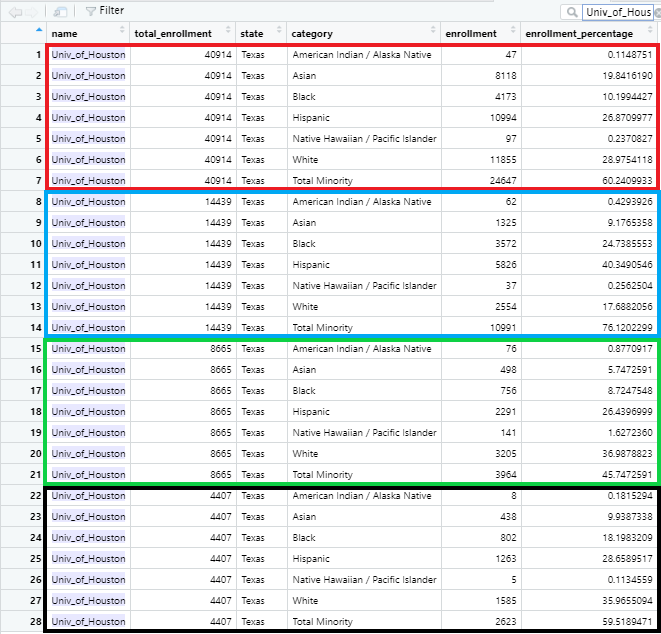
\includegraphics[width=0.75\linewidth]{Univ_of_Houston} \caption{**University of Houston Example**}\label{fig:pressure1}
\end{figure}

What we would like to do is combine each of the four into one set of 7
lines with the averages calculated for each category's enrollment and
enrollment percentage.

\hypertarget{randomly-selected-not-for-profit-educational-institutions}{%
\subsubsection{35 Randomly selected not-for-profit educational
institutions}\label{randomly-selected-not-for-profit-educational-institutions}}

For consistency of methodology we decided to select 35 schools from the
not-for-profit educational institutions to compare to the 35 randomly
selected for-profit schools. The final list of randomly selected
not-for-profit schools was also geographically diverse.

\begin{Shaded}
\begin{Highlighting}[]
\KeywordTok{sample_n}\NormalTok{(diversity_new,}\DecValTok{35}\NormalTok{)}
\end{Highlighting}
\end{Shaded}

\begin{verbatim}
## # A tibble: 35 x 6
##    name        total_enrollment state   category     enrollment enrollment_perc~
##    <chr>                  <dbl> <chr>   <chr>             <dbl>            <dbl>
##  1 Strayer Un~             2769 Florida Native Hawa~          6            0.217
##  2 Mount Oliv~             3456 North ~ American In~         15            0.434
##  3 City Colle~              575 Florida White                77           13.4  
##  4 Everest Co~              410 Washin~ Asian                29            7.07 
##  5 Kaplan Col~              435 Texas   American In~          1            0.230
##  6 ITT Techni~              330 Oklaho~ Asian                11            3.33 
##  7 Johnson & ~             1391 Colora~ Women               840           60.4  
##  8 Future Gen~               38 West V~ Native Hawa~          0            0    
##  9 University~             6811 Connec~ Total Minor~       1475           21.7  
## 10 Webster Un~            16769 Missou~ Two Or More~        314            1.87 
## # ... with 25 more rows
\end{verbatim}

\hypertarget{jennifer-1}{%
\subsubsection{Jennifer}\label{jennifer-1}}

\begin{itemize}
\tightlist
\item
  University of Idaho
\item
  Southeastern Community College (Iowa)
\item
  Clover Park Technical College
\item
  Clark College
\item
  City University of New York Hunter College
\item
  University of Houston

  \begin{itemize}
  \tightlist
  \item
    University of Houston
  \item
    University of Houston-Downtown
  \item
    University of Houston-Clear Lake
  \item
    University of Houston-Victoria
  \end{itemize}
\item
  University of Colorado

  \begin{itemize}
  \tightlist
  \item
    University of Colorado at Colorado Springs
  \item
    University of Colorado at Boulder
  \item
    University of Colorado at Denver
  \end{itemize}
\item
  University of Massachusetts

  \begin{itemize}
  \tightlist
  \item
    University of Massachusetts at Dartmouth
  \item
    University of Massachusetts at Worcester
  \item
    University of Massachusetts at Amherst
  \item
    University of Massachusetts at Lowell
  \item
    University of Massachusetts at Boston
  \end{itemize}
\item
  Arizona College

  \begin{itemize}
  \tightlist
  \item
    Arizona College at Glendale
  \item
    Arizona College at Mesa
  \end{itemize}
\item
  San Diego City College
\end{itemize}

\hypertarget{ana-1}{%
\subsubsection{Ana}\label{ana-1}}

\begin{itemize}
\tightlist
\item
  State University of New York College at Purchase
\item
  Eastern Shore Community College
\item
  Southern Oregon University
\item
  Santa Monica College
\item
  Adirondack Community College
\item
  East Georgia State College
\item
  Smith College
\item
  East Tennessee State University
\item
  Austin Community College
\item
  Tompkins Cortland Community College
\end{itemize}

\hypertarget{tiffany-1}{%
\subsubsection{Tiffany}\label{tiffany-1}}

\begin{itemize}
\tightlist
\item
  University of Hawaii Hawaii Community College
\item
  Burlington College
\item
  Pennsylvania State University - Harrisburg
\item
  University of Minnesota
\item
  University of Central Oklahoma
\item
  Southern Virginia University
\item
  Pennsylvania Highlands Community College
\item
  Arizona State University
\item
  ITT Technical Institute at Knoxville
\item
  Colgate University
\item
  University of Pittsburg
\end{itemize}

\hypertarget{jennifer-non-profit-name-changes}{%
\subsubsection{Jennifer Non-Profit Name
Changes}\label{jennifer-non-profit-name-changes}}

\begin{Shaded}
\begin{Highlighting}[]
\NormalTok{diversity_new5}\OperatorTok{$}\NormalTok{name[}\KeywordTok{grepl}\NormalTok{(}\StringTok{'University of Houston'}\NormalTok{, diversity_new5}\OperatorTok{$}\NormalTok{name)] <-}\StringTok{ 'Univ. of Houston'}

\NormalTok{diversity_new5}\OperatorTok{$}\NormalTok{name[}\KeywordTok{grepl}\NormalTok{(}\StringTok{'University of Colorado'}\NormalTok{, diversity_new5}\OperatorTok{$}\NormalTok{name)] <-}\StringTok{ 'Univ. of Colorado'}

\NormalTok{diversity_new5}\OperatorTok{$}\NormalTok{name[}\KeywordTok{grepl}\NormalTok{(}\StringTok{'University of Massachusetts'}\NormalTok{, diversity_new5}\OperatorTok{$}\NormalTok{name)] <-}\StringTok{ 'Univ. of Massachusetts'}

\NormalTok{diversity_new5}\OperatorTok{$}\NormalTok{name[}\KeywordTok{grepl}\NormalTok{(}\StringTok{'Arizona College'}\NormalTok{, diversity_new5}\OperatorTok{$}\NormalTok{name)] <-}\StringTok{ 'Arizona College'}

\NormalTok{diversity_new5}\OperatorTok{$}\NormalTok{name[}\KeywordTok{grepl}\NormalTok{(}\StringTok{'University of Idaho'}\NormalTok{, diversity_new5}\OperatorTok{$}\NormalTok{name)] <-}\StringTok{ 'Univ. of Idaho'}

\NormalTok{diversity_new5}\OperatorTok{$}\NormalTok{name[}\KeywordTok{grepl}\NormalTok{(}\StringTok{'Clark College'}\NormalTok{, diversity_new5}\OperatorTok{$}\NormalTok{name)] <-}\StringTok{ 'Clark College'}

\NormalTok{diversity_new5}\OperatorTok{$}\NormalTok{name[}\KeywordTok{grepl}\NormalTok{(}\StringTok{'City University of New York Hunter College'}\NormalTok{, diversity_new5}\OperatorTok{$}\NormalTok{name)] <-}\StringTok{ 'City Univ. New York Hunter College'}
\end{Highlighting}
\end{Shaded}

\hypertarget{ana-non-profit-name-changes}{%
\subsubsection{Ana Non-Profit Name
Changes}\label{ana-non-profit-name-changes}}

\begin{Shaded}
\begin{Highlighting}[]
\NormalTok{diversity_new5}\OperatorTok{$}\NormalTok{name[}\KeywordTok{grepl}\NormalTok{(}\StringTok{'State University of New York'}\NormalTok{, diversity_new5}\OperatorTok{$}\NormalTok{name)] <-}\StringTok{ 'State Univ. of New York'} 
\end{Highlighting}
\end{Shaded}

\hypertarget{tiffany-non-profit-name-changes}{%
\subsubsection{Tiffany Non-Profit Name
Changes}\label{tiffany-non-profit-name-changes}}

\begin{Shaded}
\begin{Highlighting}[]
\NormalTok{diversity_new5}\OperatorTok{$}\NormalTok{name[}\KeywordTok{grepl}\NormalTok{(}\StringTok{'Pennsylvania State University'}\NormalTok{,diversity_new5}\OperatorTok{$}\NormalTok{name)]<-}\StringTok{ 'Penn State Univ.'}

\NormalTok{diversity_new5}\OperatorTok{$}\NormalTok{name[}\KeywordTok{grepl}\NormalTok{(}\StringTok{'University of Minnesota'}\NormalTok{,diversity_new5}\OperatorTok{$}\NormalTok{name)]<-}\StringTok{ 'Univ. of Minn'}

\NormalTok{diversity_new5}\OperatorTok{$}\NormalTok{name[}\KeywordTok{grepl}\NormalTok{(}\StringTok{'Arizona State University'}\NormalTok{,diversity_new5}\OperatorTok{$}\NormalTok{name)]<-}\StringTok{ 'Arizona State'}

\NormalTok{diversity_new5}\OperatorTok{$}\NormalTok{name[}\KeywordTok{grepl}\NormalTok{(}\StringTok{'ITT Technical Institute'}\NormalTok{,diversity_new5}\OperatorTok{$}\NormalTok{name)]<-}\StringTok{ 'ITT Tech'} 
\end{Highlighting}
\end{Shaded}

\hypertarget{create-a-new-column-to-identify-the-randomly-selected-for-profit-colleges-sample.}{%
\subsection{Create a new column to identify the randomly selected
for-profit colleges
sample.}\label{create-a-new-column-to-identify-the-randomly-selected-for-profit-colleges-sample.}}

We were initially going to use the column to create our plots and
complete out analysis, however we realized it would be faster to create
separate datasets with the randomly selected schools. The below coding
successfully create a new column with ``1'' for the identified
for-profit colleges and ``0'' for the rest.

\hypertarget{produces-1-for-for-profit-random-selections-and-0-for-the-rest}{%
\subsubsection{Produces 1 for For-Profit Random Selections and 0 for the
rest}\label{produces-1-for-for-profit-random-selections-and-0-for-the-rest}}

\begin{Shaded}
\begin{Highlighting}[]
\NormalTok{diversity_new3 <-}\StringTok{ }\NormalTok{diversity_new }\OperatorTok\StringTok{ }\KeywordTok{mutate}\NormalTok{(diversity_new,}\DataTypeTok{forProfit =} \KeywordTok{ifelse}\NormalTok{(name}\OperatorTok{==}\StringTok{"Spencerian_College"}\NormalTok{, }\DecValTok{1}\NormalTok{,}
     \KeywordTok{ifelse}\NormalTok{(name}\OperatorTok{==}\StringTok{"Aspen University"}\NormalTok{, }\DecValTok{1}\NormalTok{, }
        \KeywordTok{ifelse}\NormalTok{(name}\OperatorTok{==}\StringTok{"American Public University system"}\NormalTok{, }\DecValTok{1}\NormalTok{, }\DecValTok{0}\NormalTok{))))}
\end{Highlighting}
\end{Shaded}

\begin{Shaded}
\begin{Highlighting}[]
\NormalTok{diversity_new3}\OperatorTok{$}\NormalTok{forProfit[}\DecValTok{47834}\NormalTok{] }\CommentTok{# Check on Spencerian_College entry}
\end{Highlighting}
\end{Shaded}

\begin{verbatim}
## [1] 0
\end{verbatim}

\begin{Shaded}
\begin{Highlighting}[]
\NormalTok{diversity_new3}\OperatorTok{$}\NormalTok{forProfit[}\DecValTok{24533}\NormalTok{] }\CommentTok{# Check on Aspen University}
\end{Highlighting}
\end{Shaded}

\begin{verbatim}
## [1] 1
\end{verbatim}

\begin{Shaded}
\begin{Highlighting}[]
\NormalTok{diversity_new3}\OperatorTok{$}\NormalTok{forProfit[}\DecValTok{123}\NormalTok{] }\CommentTok{# Check on American Public University system}
\end{Highlighting}
\end{Shaded}

\begin{verbatim}
## [1] 1
\end{verbatim}

\hypertarget{creating-a-two-new-datasets-to-compare-of-for-profit-and-not-for-profit-institutions}{%
\subsection{\texorpdfstring{\textbf{Creating a two new datasets to
compare of for-profit and not-for-profit
institutions}}{Creating a two new datasets to compare of for-profit and not-for-profit institutions}}\label{creating-a-two-new-datasets-to-compare-of-for-profit-and-not-for-profit-institutions}}

Is there a simpler way to group these?

\begin{Shaded}
\begin{Highlighting}[]
\NormalTok{for_profit2 <-}\StringTok{ }\NormalTok{diversity_new5 }\OperatorTok\StringTok{ }
\StringTok{  }\KeywordTok{filter}\NormalTok{(name }\OperatorTok{==}\StringTok{ "Spencerian College"} \OperatorTok{|}
\StringTok{           }\NormalTok{name }\OperatorTok{==}\StringTok{ "Mildred Elley"} \OperatorTok{|}\StringTok{ }
\StringTok{           }\NormalTok{name }\OperatorTok{==}\StringTok{ "Brookline College"} \OperatorTok{|}\StringTok{ }
\StringTok{           }\NormalTok{name }\OperatorTok{==}\StringTok{ "Grand Canyon Univ."} \OperatorTok{|}\StringTok{ }
\StringTok{           }\NormalTok{name }\OperatorTok{==}\StringTok{ "Aspen Univ."} \OperatorTok{|}\StringTok{ }
\StringTok{           }\NormalTok{name }\OperatorTok{==}\StringTok{ "American Public Univ."} \OperatorTok{|}\StringTok{ }
\StringTok{           }\NormalTok{name }\OperatorTok{==}\StringTok{ "Western Intl Univ."} \OperatorTok{|}\StringTok{ }
\StringTok{           }\NormalTok{name }\OperatorTok{==}\StringTok{ "NewSchool Arch. Design"} \OperatorTok{|}\StringTok{ }
\StringTok{           }\NormalTok{name }\OperatorTok{==}\StringTok{ "Schiller Intl Univ."} \OperatorTok{|}\StringTok{ }
\StringTok{           }\NormalTok{name }\OperatorTok{==}\StringTok{ "Natl Paralegal College"} \OperatorTok{|}\StringTok{ }
\StringTok{           }\NormalTok{name }\OperatorTok{==}\StringTok{ "West Coast Univ."} \OperatorTok{|}\StringTok{ }
\StringTok{           }\NormalTok{name }\OperatorTok{==}\StringTok{ "Blue Cliff College"} \OperatorTok{|}\StringTok{ }
\StringTok{           }\NormalTok{name }\OperatorTok{==}\StringTok{ "Walden University"} \OperatorTok{|}
\StringTok{           }\NormalTok{name }\OperatorTok{==}\StringTok{ "Neumont University"} \OperatorTok{|}
\StringTok{           }\NormalTok{name }\OperatorTok{==}\StringTok{ "University of Phoenix"} \OperatorTok{|}\StringTok{ }
\StringTok{           }\NormalTok{name }\OperatorTok{==}\StringTok{ "Stevens-Henager College"} \OperatorTok{|}\StringTok{ }
\StringTok{           }\NormalTok{name }\OperatorTok{==}\StringTok{ "DeVry Univ."} \OperatorTok{|}\StringTok{ }
\StringTok{           }\NormalTok{name }\OperatorTok{==}\StringTok{ "Pioneer Pacific College"} \OperatorTok{|}\StringTok{ }
\StringTok{           }\NormalTok{name }\OperatorTok{==}\StringTok{ "Stratford University"} \OperatorTok{|}\StringTok{ }
\StringTok{           }\NormalTok{name }\OperatorTok{==}\StringTok{ "Capella University"} \OperatorTok{|}\StringTok{ }
\StringTok{           }\NormalTok{name }\OperatorTok{==}\StringTok{ "Grantham University"} \OperatorTok{|}\StringTok{ }
\StringTok{           }\NormalTok{name }\OperatorTok{==}\StringTok{ "Redstone College"} \OperatorTok{|}\StringTok{ }
\StringTok{           }\NormalTok{name }\OperatorTok{==}\StringTok{ "National College"} \OperatorTok{|}\StringTok{ }
\StringTok{           }\NormalTok{name }\OperatorTok{==}\StringTok{ "Strayer Univ."} \OperatorTok{|}\StringTok{ }
\StringTok{           }\NormalTok{name }\OperatorTok{==}\StringTok{ "Lincoln Tech"} \OperatorTok{|}\StringTok{ }
\StringTok{           }\NormalTok{name }\OperatorTok{==}\StringTok{ "Fashion Institute"} \OperatorTok{|}\StringTok{ }
\StringTok{           }\NormalTok{name }\OperatorTok{==}\StringTok{ "Centura College"} \OperatorTok{|}\StringTok{  }
\StringTok{           }\NormalTok{name }\OperatorTok{==}\StringTok{ "Rasmussen College"} \OperatorTok{|}\StringTok{ }
\StringTok{           }\NormalTok{name }\OperatorTok{==}\StringTok{ "Fortis College"} \OperatorTok{|}\StringTok{ }
\StringTok{           }\NormalTok{name }\OperatorTok{==}\StringTok{ "Full Sail University"} \OperatorTok{|}\StringTok{ }
\StringTok{           }\NormalTok{name }\OperatorTok{==}\StringTok{ "Rocky Mountain College of Art & Design"} \OperatorTok{|}\StringTok{ }
\StringTok{           }\NormalTok{name }\OperatorTok{==}\StringTok{ "Minneapolis Business College"} \OperatorTok{|}\StringTok{ }
\StringTok{           }\NormalTok{name }\OperatorTok{==}\StringTok{ "Paier College of Art"} \OperatorTok{|}\StringTok{ }
\StringTok{           }\NormalTok{name }\OperatorTok{==}\StringTok{ "Vista College"} \OperatorTok{|}\StringTok{ }
\StringTok{           }\NormalTok{name }\OperatorTok{==}\StringTok{ "Bay State College"}\NormalTok{ )}
\end{Highlighting}
\end{Shaded}

\begin{Shaded}
\begin{Highlighting}[]
\KeywordTok{str}\NormalTok{(for_profit2)}
\end{Highlighting}
\end{Shaded}

\begin{verbatim}
## tibble [1,183 x 6] (S3: spec_tbl_df/tbl_df/tbl/data.frame)
##  $ name                 : chr [1:1183] "University of Phoenix" "University of Phoenix" "University of Phoenix" "University of Phoenix" ...
##  $ total_enrollment     : num [1:1183] 195059 195059 195059 195059 195059 ...
##  $ state                : chr [1:1183] "Arizona" "Arizona" "Arizona" "Arizona" ...
##  $ category             : chr [1:1183] "American Indian / Alaska Native" "Asian" "Black" "Hispanic" ...
##  $ enrollment           : num [1:1183] 876 1959 31455 13984 1019 ...
##  $ enrollment_percentage: num [1:1183] 0.449 1.004 16.126 7.169 0.522 ...
##  - attr(*, "spec")=
##   .. cols(
##   ..   name = col_character(),
##   ..   total_enrollment = col_double(),
##   ..   state = col_character(),
##   ..   category = col_character(),
##   ..   enrollment = col_double()
##   .. )
\end{verbatim}

\begin{Shaded}
\begin{Highlighting}[]
\KeywordTok{head}\NormalTok{(for_profit2)}
\end{Highlighting}
\end{Shaded}

\begin{verbatim}
## # A tibble: 6 x 6
##   name       total_enrollment state  category       enrollment enrollment_perce~
##   <chr>                 <dbl> <chr>  <chr>               <dbl>             <dbl>
## 1 Universit~           195059 Arizo~ American Indi~        876             0.449
## 2 Universit~           195059 Arizo~ Asian                1959             1.00 
## 3 Universit~           195059 Arizo~ Black               31455            16.1  
## 4 Universit~           195059 Arizo~ Hispanic            13984             7.17 
## 5 Universit~           195059 Arizo~ Native Hawaii~       1019             0.522
## 6 Universit~           195059 Arizo~ White               58209            29.8
\end{verbatim}

\begin{Shaded}
\begin{Highlighting}[]
\NormalTok{not_profit <-}\StringTok{ }\NormalTok{diversity_new5 }\OperatorTok\StringTok{ }
\StringTok{  }\KeywordTok{filter}\NormalTok{(name }\OperatorTok{==}\StringTok{ "Univ. of Idaho"} \OperatorTok{|}
\StringTok{           }\NormalTok{total_enrollment }\OperatorTok{==}\StringTok{ "2987"}\OperatorTok{|}
\StringTok{           }\NormalTok{name }\OperatorTok{==}\StringTok{ "Clover Park Technical College"}\OperatorTok{|}
\StringTok{           }\NormalTok{name }\OperatorTok{==}\StringTok{ "Clark College"}\OperatorTok{|}
\StringTok{           }\NormalTok{name }\OperatorTok{==}\StringTok{ "City Univ. New York Hunter College"}\OperatorTok{|}
\StringTok{           }\NormalTok{name }\OperatorTok{==}\StringTok{ "Univ. of Houston"} \OperatorTok{|}\StringTok{ }
\StringTok{           }\NormalTok{name }\OperatorTok{==}\StringTok{ "Univ. of Colorado"}\OperatorTok{|}
\StringTok{           }\NormalTok{name }\OperatorTok{==}\StringTok{ "Univ. of Massachusetts"} \OperatorTok{|}
\StringTok{           }\NormalTok{name }\OperatorTok{==}\StringTok{ "Arizona College"} \OperatorTok{|}
\StringTok{           }\NormalTok{name }\OperatorTok{==}\StringTok{ "San Diego City College"} \OperatorTok{|}\StringTok{ }
\StringTok{           }\NormalTok{name }\OperatorTok{==}\StringTok{ "State Univ. of New York"} \OperatorTok{|}\StringTok{ }
\StringTok{           }\NormalTok{name }\OperatorTok{==}\StringTok{ "Eastern Shore Community College"} \OperatorTok{|}\StringTok{ }
\StringTok{           }\NormalTok{name }\OperatorTok{==}\StringTok{ "Southern Oregon University"} \OperatorTok{|}\StringTok{ }
\StringTok{           }\NormalTok{name }\OperatorTok{==}\StringTok{ "Santa Monica College"} \OperatorTok{|}\StringTok{ }
\StringTok{           }\NormalTok{name }\OperatorTok{==}\StringTok{ "Adirondack Community College"} \OperatorTok{|}\StringTok{ }
\StringTok{           }\NormalTok{name }\OperatorTok{==}\StringTok{ "East Georgia State College"} \OperatorTok{|}\StringTok{ }
\StringTok{           }\NormalTok{name }\OperatorTok{==}\StringTok{ "Smith College"} \OperatorTok{|}\StringTok{ }
\StringTok{           }\NormalTok{name }\OperatorTok{==}\StringTok{ "East Tennessee State University"} \OperatorTok{|}\StringTok{ }
\StringTok{           }\NormalTok{name }\OperatorTok{==}\StringTok{ "Austin Community College"} \OperatorTok{|}\StringTok{ }
\StringTok{           }\NormalTok{name }\OperatorTok{==}\StringTok{ "Tompkins Cortland Community College"} \OperatorTok{|}\StringTok{ }
\StringTok{           }\NormalTok{name }\OperatorTok{==}\StringTok{ "Penn State Univ."} \OperatorTok{|}\StringTok{ }
\StringTok{           }\NormalTok{name }\OperatorTok{==}\StringTok{ "Univ. of Minn"} \OperatorTok{|}\StringTok{ }
\StringTok{           }\NormalTok{name }\OperatorTok{==}\StringTok{ "Arizona State"} \OperatorTok{|}\StringTok{ }
\StringTok{           }\NormalTok{name }\OperatorTok{==}\StringTok{ "ITT Tech"} \OperatorTok{|}\StringTok{ }
\StringTok{           }\NormalTok{name }\OperatorTok{==}\StringTok{ "University of Hawaii Hawaii Community College"} \OperatorTok{|}\StringTok{ }
\StringTok{           }\NormalTok{name }\OperatorTok{==}\StringTok{ "Burlington College"} \OperatorTok{|}\StringTok{ }
\StringTok{           }\NormalTok{name }\OperatorTok{==}\StringTok{ "University of Central Oklahoma"} \OperatorTok{|}\StringTok{ }
\StringTok{           }\NormalTok{name }\OperatorTok{==}\StringTok{ "Southern Virginia University"} \OperatorTok{|}\StringTok{ }
\StringTok{           }\NormalTok{name }\OperatorTok{==}\StringTok{ "Pennsylvania Highlands Community College"} \OperatorTok{|}\StringTok{ }
\StringTok{           }\NormalTok{name }\OperatorTok{==}\StringTok{ "Colgate University"}\OperatorTok{|}
\StringTok{           }\NormalTok{name }\OperatorTok{==}\StringTok{ "University of Pittsburg"}\NormalTok{)}
\end{Highlighting}
\end{Shaded}

For some reason the name filter for ``Southeastern Community College
(Iowa)'' would not select properly. The same happened for the attempted
name change above.

\hypertarget{visualizations}{%
\subsection{\texorpdfstring{\textbf{Visualizations}}{Visualizations}}\label{visualizations}}

\begin{Shaded}
\begin{Highlighting}[]
\KeywordTok{head}\NormalTok{(not_profit)}
\end{Highlighting}
\end{Shaded}

\begin{verbatim}
## # A tibble: 6 x 6
##   name     total_enrollment state   category        enrollment enrollment_perce~
##   <chr>               <dbl> <chr>   <chr>                <dbl>             <dbl>
## 1 Univ. o~            51147 Minnes~ American India~        163            0.319 
## 2 Univ. o~            51147 Minnes~ Asian                 3998            7.82  
## 3 Univ. o~            51147 Minnes~ Black                 1785            3.49  
## 4 Univ. o~            51147 Minnes~ Hispanic              1544            3.02  
## 5 Univ. o~            51147 Minnes~ Native Hawaiia~         31            0.0606
## 6 Univ. o~            51147 Minnes~ White                33674           65.8
\end{verbatim}

\begin{Shaded}
\begin{Highlighting}[]
\KeywordTok{library}\NormalTok{(ggplot2)}
\end{Highlighting}
\end{Shaded}

\begin{Shaded}
\begin{Highlighting}[]
\NormalTok{plot1 <-}\StringTok{ }\NormalTok{for_profit2 }\OperatorTok
\StringTok{  }\KeywordTok{ggplot}\NormalTok{() }\OperatorTok{+}
\StringTok{  }\KeywordTok{geom_bar}\NormalTok{(}\KeywordTok{aes}\NormalTok{(}\DataTypeTok{x=}\NormalTok{name, }\DataTypeTok{y=}\NormalTok{ enrollment_percentage , }
              \DataTypeTok{fill =}\NormalTok{ category),}
              \DataTypeTok{position =} \StringTok{"fill"}\NormalTok{, }
              \DataTypeTok{stat =} \StringTok{"identity"}\NormalTok{ ) }\OperatorTok{+}
\StringTok{  }\KeywordTok{coord_flip}\NormalTok{() }\OperatorTok{+}
\StringTok{  }\KeywordTok{theme_minimal}\NormalTok{() }\OperatorTok{+}
\StringTok{  }\KeywordTok{ggtitle}\NormalTok{(}\StringTok{"Diversity Percent of Enrollment in For Profit US Schools"}\NormalTok{, ) }\OperatorTok{+}
\StringTok{  }\KeywordTok{theme}\NormalTok{ (}\DataTypeTok{plot.title =} \KeywordTok{element_text}\NormalTok{(}\DataTypeTok{hjust =} \FloatTok{.01}\NormalTok{, }\DataTypeTok{size=}\DecValTok{12}\NormalTok{)) }\OperatorTok{+}
\StringTok{  }\KeywordTok{labs}\NormalTok{(}\DataTypeTok{fill =} \StringTok{"Race"}\NormalTok{) }\OperatorTok{+}
\StringTok{  }\KeywordTok{theme}\NormalTok{(}\DataTypeTok{legend.justification =} \DecValTok{-5}\NormalTok{, }
        \DataTypeTok{legend.position=}\StringTok{"bottom"}\NormalTok{, }
        \DataTypeTok{legend.text =} \KeywordTok{element_text}\NormalTok{(}\DataTypeTok{size=}\DecValTok{6}\NormalTok{) ,}
\NormalTok{        )  }\OperatorTok{+}
\StringTok{  }\KeywordTok{theme}\NormalTok{(}\DataTypeTok{axis.text.y =} \KeywordTok{element_text}\NormalTok{(}\DataTypeTok{size =} \DecValTok{7}\NormalTok{)) }\OperatorTok{+}
\StringTok{  }\KeywordTok{xlab}\NormalTok{(}\StringTok{"School Name"}\NormalTok{) }\OperatorTok{+}
\StringTok{  }\KeywordTok{ylab}\NormalTok{ (}\StringTok{"Percent of Enrollment"}\NormalTok{) }
\NormalTok{plot1}
\end{Highlighting}
\end{Shaded}

\includegraphics{final_project_8.10_files/figure-latex/unnamed-chunk-58-1.pdf}

\begin{Shaded}
\begin{Highlighting}[]
\NormalTok{plot2 <-}\StringTok{ }\NormalTok{not_profit }\OperatorTok
\StringTok{  }\KeywordTok{ggplot}\NormalTok{() }\OperatorTok{+}
\StringTok{  }\KeywordTok{geom_bar}\NormalTok{(}\KeywordTok{aes}\NormalTok{(}\DataTypeTok{x=}\NormalTok{name, }\DataTypeTok{y=}\NormalTok{ enrollment_percentage , }
              \DataTypeTok{fill =}\NormalTok{ category),}
              \DataTypeTok{position =} \StringTok{"fill"}\NormalTok{, }
              \DataTypeTok{stat =} \StringTok{"identity"}\NormalTok{ ) }\OperatorTok{+}
\StringTok{  }\KeywordTok{coord_flip}\NormalTok{() }\OperatorTok{+}
\StringTok{  }\KeywordTok{theme_minimal}\NormalTok{() }\OperatorTok{+}
\StringTok{  }\KeywordTok{ggtitle}\NormalTok{(}\StringTok{"Diversity Percent of Enrollment in Not for Profit US Schools"}\NormalTok{, ) }\OperatorTok{+}
\StringTok{  }\KeywordTok{theme}\NormalTok{ (}\DataTypeTok{plot.title =} \KeywordTok{element_text}\NormalTok{(}\DataTypeTok{hjust =} \FloatTok{.01}\NormalTok{, }\DataTypeTok{size=}\DecValTok{11}\NormalTok{)) }\OperatorTok{+}
\StringTok{  }\KeywordTok{labs}\NormalTok{(}\DataTypeTok{fill =} \StringTok{"Race"}\NormalTok{) }\OperatorTok{+}
\StringTok{  }\KeywordTok{theme}\NormalTok{(}\DataTypeTok{legend.position=}\StringTok{"bottom"}\NormalTok{, }
        \DataTypeTok{legend.justification =} \StringTok{"left"}\NormalTok{,}
        \DataTypeTok{legend.text =} \KeywordTok{element_text}\NormalTok{(}\DataTypeTok{size=}\DecValTok{6}\NormalTok{) ,}
\NormalTok{        )  }\OperatorTok{+}
\StringTok{  }\KeywordTok{xlab}\NormalTok{(}\StringTok{"School Name"}\NormalTok{) }\OperatorTok{+}
\StringTok{  }\KeywordTok{ylab}\NormalTok{ (}\StringTok{"Percent of Enrollment"}\NormalTok{) }
\NormalTok{plot2}
\end{Highlighting}
\end{Shaded}

\includegraphics{final_project_8.10_files/figure-latex/unnamed-chunk-59-1.pdf}

\hypertarget{data-analysis}{%
\subsection{\texorpdfstring{\textbf{Data
Analysis}}{Data Analysis}}\label{data-analysis}}

As the graphs above illustrate, our data verifies that indeed there are
a higher proportion of students of color at for-profit colleges than at
non-profit colleges. White Students (shown in pink in the above plots)
have much greater attendance at non-profit colleges. These findings
provide support for the argument that there are higher numbers of
enrollment of students of color at for-profit colleges. One possible
explanation could be targeted marketing campaigns by for-profit colleges
to students of color. Further research is required.

Given the well-documented high cost of for-profit education, the
exorbitant student debt incurred at these schools, the lower rates of
employment upon graduation and the low levels of satisfaction with
educational quality from previous students, all potential students
should think twice before enrolling in for-profit colleges. This is
particularly true for students of color who may be identified by
for-profit colleges as susceptible to predatory exploitative practices
that will provide additional profits to the college's shareholders
without making good on their promise to provide a marketable, quality
education. The predatory actions of for-profit colleges contribute to
our nation's growing economic divide between the haves and the have nots
and perpetuates the unequal education system we have today. Fortunately,
there are many people and organizations working to end these predatory
practices, but in the meantime while they continue to exist, we must
inform one another about the importance of obtaining a quality education
at not-for-profit institutions, like Montgomery College.

\hypertarget{future-research}{%
\subsection{\texorpdfstring{\textbf{Future
Research}}{Future Research}}\label{future-research}}

The following is a list of more detailed analysis that could be done
with this dataset:

\begin{enumerate}
\def\labelenumi{\arabic{enumi}.}
\item
  Comparing diversity of for-profit and not-for-profit schools in the
  same geographic regions utilizing local racial demographics.
\item
  Comparing community colleges, to four-year-institutions, to for-profit
  institutions
\item
  Comparing the tuition rates, salary potential and overall profits
  received from community colleges, four-year institutions and
  for-profit institutions.
\item
  A longitudinal study could be conducted to see if there have been
  changes in the demographic makeup of for-profit colleges in the time
  before the Obama-era regulations, the lack of regulation during the
  DeVos era and the patterns that emerge after the predatory lending
  lawsuits and any resulting legislation.
\end{enumerate}

\hypertarget{references}{%
\subsection{\texorpdfstring{\textbf{References}}{References}}\label{references}}

Body, D. (2019, Mar.~19). Worse Off Than When They Enrolled: The
Consequence of For-Profit Colleges for People of Color. \emph{The Aspen
Institute}.
\url{https://www.aspeninstitute.org/blog-posts/worse-off-than-when-they-enrolled-the-consequence-of-for-profit-colleges-for-people-of-color/}

Bonadies, G.G., Rovenger, J., Connor, E., Shum, B. \& Merrill, T. (2018,
Jul.~30). For-Profit Schools' Predatory Practices and Students of Color:
A Mission to Enroll Rather than Educate, \emph{Harvard Law Review Blog}.
\url{https://blog.harvardlawreview.org/for-profit-schools-predatory-practices-and-students-of-color-a-mission-to-enroll-rather-than-educate/}

Conti, A. (2019, Sep.~10). How For-Profit Colleges Have Targeted and
Taken Advantage of Black Students. \emph{Vice}.
\url{https://www.vice.com/en_us/article/bjwj3d/how-for-profit-colleges-have-targeted-and-taken-advantage-of-black-students}

Green, E.L. (2019, Jun.~28). DeVos Repeals Obama-Era Rule Cracking down
on For-Profit Colleges, \emph{New York Times}.
\url{https://www.nytimes.com/2019/06/28/us/politics/betsy-devos-for-profit-colleges.html}

Halperin, D. 22 States Sue DeVos to Overturn Anti-Student Rule.
\emph{Republic Report}.
\url{https://www.republicreport.org/2020/22-states-sue-devos-to-overturn-anti-student-rule/}

Legal Services Center(2020), \emph{Project on Predatory Student Lending:
Cases}, Harvard Law School.
\url{https://predatorystudentlending.org/cases/}

Lobosco, K. (2019, Jul.~23). For-profit college students are waiting 958
days for loan relief, \emph{CNN}.
\url{https://www.cnn.com/2019/07/23/politics/betsy-devos-loan-forgiveness-for-profit-college-students/index.html}

Lopez, M. (2015, Feb.~12). BEWARE: For-Profit Colleges. \emph{The
Patriot Post}.
\url{https://bcchspatriotpost.com/2391/news/beware-for-profit-colleges/}

Redman, H. (2020, Jun.~27). AG Sues Department of Education Over
For-Profit College Rules. \emph{Urban Milwaukee}.
\url{https://urbanmilwaukee.com/2020/06/27/ag-sues-department-of-education-over-for-profit-college-rules/}

TBS Staff (2019, Jul.~29). For-Profit Colleges vs.~Non-Profit Colleges -
What's The Difference? \emph{The Best Schools Magazine}.
\url{https://thebestschools.org/magazine/for-profit-vs-non-profit}

Turner, C. (2019, Nov.~14). Devos Refuses to Forgive student Debt For
Those DeFrauded by For-Profit Colleges, \emph{All Things Considered,
NPR}.
\url{https://www.npr.org/2019/11/14/779465130/devos-refuses-to-forgive-student-debt-for-those-defrauded-by-for-profit-colleges}

Voorhees, K. (2019, Oct.~17). Civil Rights Groups: For-Profit Colleges
Exploit Black and Latino Students. \emph{The Leadership Conference
Education Fund}.
\url{https://civilrights.org/edfund/2019/10/17/civil-rights-groups-for-profit-colleges-exploit-black-and-latino-students/}

\end{document}
